\documentclass[../../thesis.tex]{subfiles}

\graphicspath{{./img/}}

\begin{document}
\section{Introduction}
\label{sec: bitcoin_introduction}



The spirit of the Cypherpunk movement is to resist government interference with public privacy. Money is one of the aspects where government interferes a lot. Everything purchased online passes through a third party, e.g., a bank or a credit card company, which takes a cut from the transaction and can reject it for whatever reason. Additionally, people are cornered in an era where the only means of exchange, with privacy, is doing barter, because the whole financial system is monitored, regulated and adulterated for political reasons. This seems to be a frustrating and disappointing era for any Cypherpunk. For those who follow such ideals, the creation of means of exchange with privacy is the the final goal. Luckily, on 31 October 2008, a link to a paper authored by Satoshi Nakamoto titled \textit{Bitcoin: A Peer-to-Peer Electronic Cash System}\cite{nakamoto2008bitcoin} was posted to a cryptography mailing list\cite{satoshiMail1}\cite{satoshiMail2}. 

In his article, he detailed methods of using a fully peer-to-peer network of computers to generate a new electronic cash system, with no trusted third party. At that day the Cypherpunks observed that a new era, one of freedom and privacy, was born. On January 2009, the bitcoin network came into existence with the release of the first open source Bitcoin client and the issuance of the first Bitcoins \cite{V1Bitcoin1}\cite{V1Bitcoin2}\cite{V1Bitcoin3}. On that day, the founder placed an important message indicating the true intent behind what he had just created.
\begin{quotation}
  The Times 03/Jan/2009 Chancellor on brink of second bailout for banks.
\end{quotation}

The London Times ran a cover story titled \textit{"Chancellor on Brink of Second Bailout for Banks"}\cite{theTimes}. This title was embedded into the very first transaction ever to be included in the new Bitcoin blockchain\cite{bitcoinGenesis}, by Satoshi Nakamoto. This proved that the first block was mined after 3 January 2009, since that headline was not available before that time. The headline marks a moment where the Government of the United Kingdom planned to give a second financial assistance to the failing Banks in England to save them from collapse. Measure pumped billions of sterling pounds more into the selected bank's treasury. It is more evidence that the market was desperate and seeking a solution. The only problem was: they were looking for the wrong resolution. As \textit{Murray Rothbard} states in his essay \textit{Economic Depressions: Their Cause and Cure} \cite{rothbard2009economic}:
 \begin{quotation}
  Almost all economists of the present day, treated the economy as a potentially workable, but always troublesome and rebellious patient, with a constant tendency to get into higher inflation or unemployment. Then, the function of the government is to be the wise old manager.
\end{quotation}
We saw in 2008 that governments were not so good \textit{"wise"} managers, from all the chaotic 2008 depression. Bitcoin was born as an escape for those who want to keep the rewards of their hard work safe and away from greedy self-interested politicians. 

Bitcoin was designed to be a digital encrypted money and to remove the need of central agencies. Early inventions of digital money like Bitgold\cite{szabo2008bit} or B-money\cite{dai1998b} were never implemented or relied on a central authority like Ecash\cite{chaum1995introduction}. The most important challenging to solve without a central authority was the double-spending problem. How do we prove that a user that has paid for something with a specific coin has not used that same coin to buy something else at the same time, without having a central authority to monitor and approve the transactions? By solving these issues, Bitcoin became the very first successful decentralized digital currency. Instead of one central controlling party recording every transaction in one central ledger, all the users of the currency keep and record all of the transactions at the same time. Thus, as a result, any attempt to trick the community would be noticed since the community will verify this transaction and reject it. No one user, government or a bank can control the ledger. Bitcoin is an immutable open, decentralized ledger with censorship resistance maintained by a network of computers over the internet where anyone at any time can access that information. Using Bitcoin, users can transfer their money worldwide in a matter of minutes by paying a small fee. 



\section{How Bitcoin Works}
\label{sec:bitcoin_works}

 The Bitcoin protocol insures that the total supply of Bitcoins remains fixed, by making it impossible to copy Bitcoins or to create more Bitcoins than is previously coded. The Bitcoin rules are formulated in the source code, and all computers which run the Bitcoin software maintain the validity of the rules and keep a copy of the ledger. Meaning all machines that keep the network running must agree on the same rules. Thus, this mechanism of decentralization of the computers is what guarantees the trust of the system. The Bitcoin open source core repository provides two types of software: the full node, and the mining node, both software are available for free and both software validates the Bitcoin protocol. Bitcoin protocol acts as a decentralized ledger where every machine running the protocol has a copy of the ledger, we call this ledger, the Blockchain.

\section{Wallets}
\label{sec:bitcoin_wallet}
Besides, the full node and mining node softwares, there are another piece of software, the Wallet. To start using Bitcoin, you must download a Bitcoin Wallet. Wallets are not a type of node, and they are not responsible for maintaining the system, they act as a consumer of the network, and its primary task is to create an address, sign a transaction and broadcast it to the Bitcoin Network. Typically, a wallet transmits a transaction to a full node which is maintained by the wallet provider. They are made to work on regular commercial computers and do not run any high energy consumption computation.

By generating an address, the user of the wallet now possesses (1) a private key, which acts as a key that unlocks his funds, and (2) a public key which serves as the router number of a bank account, the information that the user needs to provide to someone in order to receive a payment. Bear in mind that a wallet must keep the private key safe on the client computer and must never broadcast that information. Only the public key is transmitted and recorded in the ledger. 


\section{Addresses}
\label{sec:bitcoin_address}

A wallet is the software responsible for generating Bitcoin addresses. The process of creating a Bitcoin Address starts by producing a 256 bits random number. This number will generate a private key and a public key. The private key produces the public key using an \textit{Elliptical Curve Function} which guarantees that the same private key will always generate the same public key, and that the matching private key is difficult to discover using only the public key. The private key must be generated using good randomness. Otherwise, it is possible that someone discovers the random number which generated the private key.

The address generated from the public key is what you use to send and receive bitcoins. It is called the Bitcoin Address. The Public keys are hashed using the \textit{SHA 256 Hash Algorithm}, and the output is hashed using the \textit{MD160 Hashing Algorithm} which results in a 160 bits Public Key Hash. Afterwards, the \textit{Base 58 Check Algorithm} encodes it to a 34 characters string that is more human readable. This also excludes the characters:  \textit{0OIl}; the number zero, capital letter "o", capital letter "i" and low case "l" to avoid human mistakes. For the sake of simplification, we will name Bitcoin address as public key since this terminology is most popular among Bitcoin users. We can see on Figure \ref{fig:key} a diagram of this process simplified.

\begin{figure}[H]
\centering

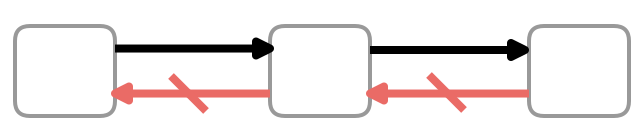
\includegraphics[width=\textwidth]{content/bitcoin/img/key}
\caption{The generation process of a Bitcoin Address. Private Key is generated from a 256 bits random number. Sequentially, using the private key as input, the \textit{Elliptical Curve function} outputs the Public Key. Finally, utilizing the public key as input, the \textit{SHA 256 Hash Algorithm}  output goes to the \textit{MD160 Hashing Algorithm} which results in a 160 bits Public Key Hash. Then, the \textit{Base 58 Check Algorithm} encodes this a 34 characters string more human readable and presentable form, where it excludes the characters:  \textit{0OIl}; the number zero, capital letter "o", capital letter "i" and low case "l" to avoid human mistakes. The result of this process is a Bitcoin Address. The red arrows indicate that the inverse process is not possible. }
\label{fig:key}
\end{figure}


\section{Blockchain}
\label{sec:blockchain}

Bitcoin broadcasts a transaction to be included in the ledger in the form of a block. A block is a data structure which acts like a bucket by collecting several incoming new transactions. A block also has a reference to its parent block, and that parent block has a reference to its parent block and so on. This collection of references of blocks is called the \textit{Blockchain}. The Blockchain is an ordered, back-linked list of blocks of transactions. The figure \ref{fig:blockchain} Represents the blockchain in a visual way, where a Block has: its hash, the previous blocks' hash, and its list of transactions. The previous block hash field creates the actual chain between the blocks. Thus, Block 12 is linked back to Black 11, and Block 11 is connected to Block 10. 

\begin{figure}[H]
\centering
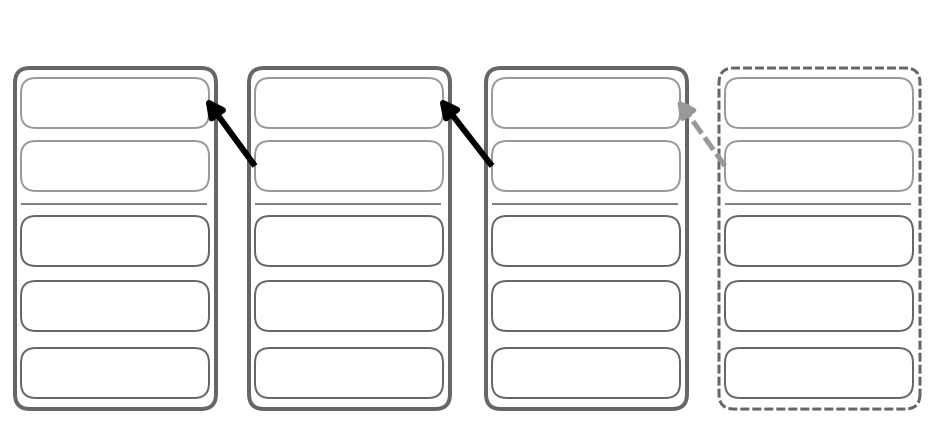
\includegraphics[width=\textwidth]{content/bitcoin/img/blockchain}
\caption{Graphical representation of the Bitcoin Blockchain Data Structure. Every Block has its hash, the previous block hash, and its list of transactions. The previous block hash field ensures the chain of blocks. Thus, Block 12 is linked back to Black 11, and Block 11 is connected to Block 10. Block 13 represents a new mined block about to be inserted to the chain. }
\label{fig:blockchain}
\end{figure}

\section{Mining Bitcoins}
\label{sec:bitcoin_mining}

New blocks are added to the blockchain by so-called "mining nodes". Mining nodes are machines running the Bitcoin mining software. This mining software is usually run on specialized computers. Mining nodes are responsible for continuously receiving new transactions from the network and validating all transactions by checking the integrity of the Bitcoin rules. Thus, mining contributes to the security of the network by accepting valid transactions or rejecting invalid transactions. However, \textit{there is no free lunch} and keeping those computers working for the network by validating the transactions has a cost. This validation job requires the miners to solve a hard computation task which uses electricity. The reward for this work is the ability of a miner to create new Bitcoins. For each block mined, the miners are rewarded with a certain amount of Bitcoins. How much is the miner rewarded for mining a block? How much Bitcoins will ever be created? How hard is the problem that must be solved? These rules of the Bitcoin network can be seen in more details in \url{https://en.bitcoin.it/wiki/Main_Page}.

We can see in Figure \ref{fig:blockchain} the representation of a new mined block (Block 13) about to be inserted into the Blockchain. This block will be included in the final state of the Blockchain only if the majority of full nodes on the network approve the validity of this block. Remember that every participant of the network keeps a copy of the Blockchain. Thus, the addition of the local copy Blockchain of the miner must be broadcasted to the others and validated by them. Figure \ref{fig:blocks_flowchart} exemplifies the process of adding a new block to the Blockchain.  In order for a newly mined block to be accepted in the final blockchain state, the full nodes must validate this block against the rules of the protocol. If the majority of the full nodes validate this block as correct, then this block is accepted and added to the final Blockchain state and broadcast to the other nodes. If the majority finds an inconsistency, then this block is rejected. However, if the nodes do not reach a consensus, this results in a rupture of the protocol, where part of the participants agree on a set of rules and another part agrees on another arrangement. This break of consensus is called a \textit{Hard fork}, which leads to a bifurcation of Blockchain, and these two chains continue to be maintained by the same network. These two chains share the same past but differ in the future from the moment of the split. 


\begin{figure}[H]
\centering
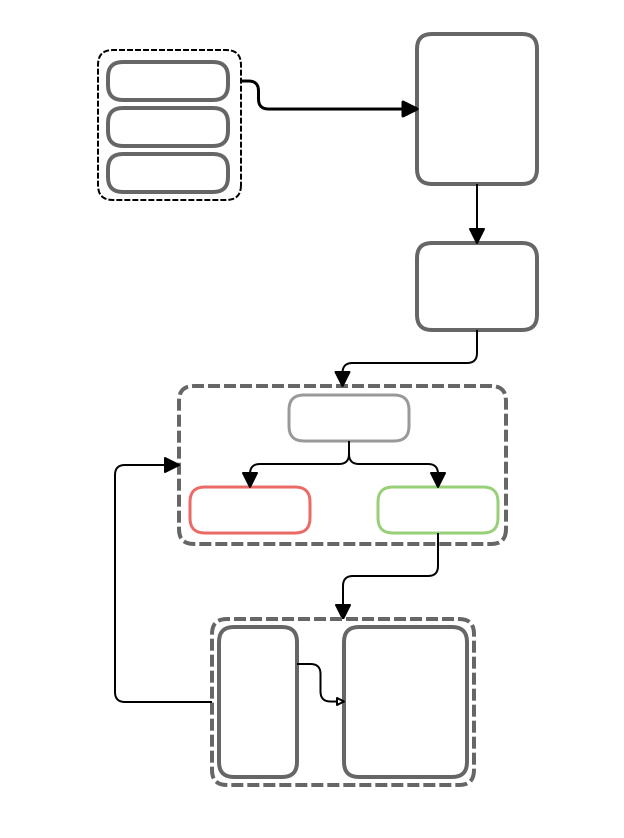
\includegraphics[width=\textwidth]{content/bitcoin/img/blocks_flowchart}
\caption{Bitcoin Mining Flowchart: process of adding a new block to the Blockchain.  In order for a newly mined block to be accepted to the final blockchain state, the full nodes must validate this block against the rules of the protocol. If the majority of the full nodes validate this block as correct, then this block is accepted and added to the final Blockchain state and broadcasted to the other nodes. If the majority finds an inconsistency, then this block is rejected. }
\label{fig:blocks_flowchart}
\end{figure}

\section{Full Node}
\label{sec:bitcoin_full_node}

A full node is a \textit{watchmen} of the miners. It has the responsibility to check if the block created by the miner follows the Bitcoin rules. If the miner of newly generated block added more Bitcoin than what is allowed, full nodes would check this block, and then mark this block as invalid. Since every node on the network has the same information, the other full nodes will achieve the same result as the first full node. Then a consensus would be reached about this invalid block. Thus, this block will not be included in the final state of the \textit{Blockchain}. The full node software does not require the same computation power as the mining node, for that reason the network does not reward full nodes. Figure \ref{fig:bitcoin_network} illustrates the overview of the Bitcoin network. The network is a combination of machines running the full nodes and miner nodes software. Each node keeps a local copy of the final state of the Blockchain; they are responsible for maintaining the network. However, only miners are allowed to modify the Blockchain state. Finally, the wallets are the end consumers of the network. They are responsible for creating Bitcoin addresses and broadcasting transactions among the addresses.



\begin{figure}[H]
\centering
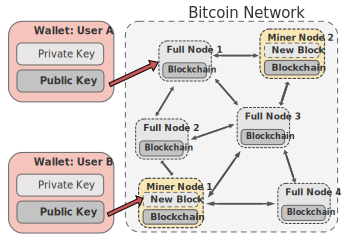
\includegraphics[width=\textwidth]{content/bitcoin/img/bitcoin_network}
\caption{Bitcoin Network Overview: a combination of machines running the full nodes and miner nodes software.
}
\label{fig:bitcoin_network}
\end{figure}

\section{Transactions}
\label{sec:bitcoin_transactions}

As stated on the Bitcoin wiki page, \begin{quotation}
  A transaction is a transfer of Bitcoin value that is broadcast to the network and collected into blocks.
\end{quotation}
 Since transactions are transmitted and recorded on the Blockchain, they are public information, meaning, they are not encrypted.  A Transaction is a transfer of ownership from one public key (i.e. address) to another. It typically contains several inputs and two outputs. An input is a reference to the old owner address from a previous transaction. Thus, inputs reference the outputs of previous transactions. Furthermore, an output is a reference to the new owners' address; this address will now hold a balance made by the transaction. Figure~\ref{fig:transactions1} helps to understand the relationship between the inputs and outputs of a transaction. Because of this reference, we can calculate the available Bitcoin balance of an address by looking at all past transactions on the Blockchain where the target address appears as output. The balance will be the sum of all the values found. 
 
 As we can see in Figure \ref{fig:transactions2}, the available balance of the wallet is the sum of the output values located on transaction A and transaction B. Note that a wallet can generate several public keys from the same private key, in this case, address C and address E belong to the same private key. The final balance of Address G is 2 Bitcoins.
 
\begin{figure}[H]
\centering
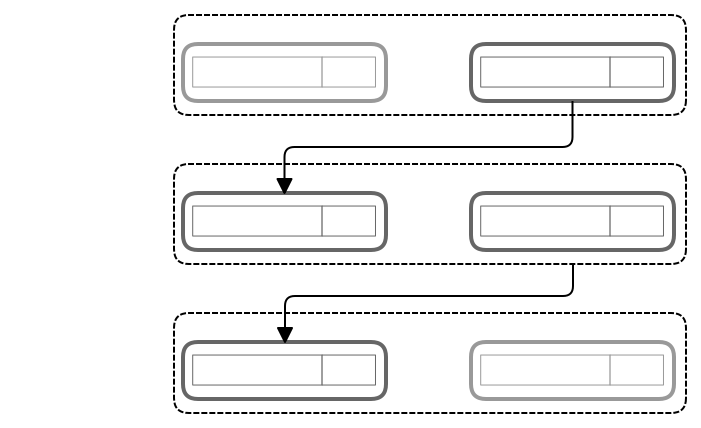
\includegraphics[width=\textwidth]{content/bitcoin/img/transactions1}
\caption{The input of transaction C is the output of transaction B meaning address C used the funds received from address B to send to address E. Analogously, transaction B with transaction A.}
\label{fig:transactions1}
\end{figure}



\begin{figure}[H]
\centering
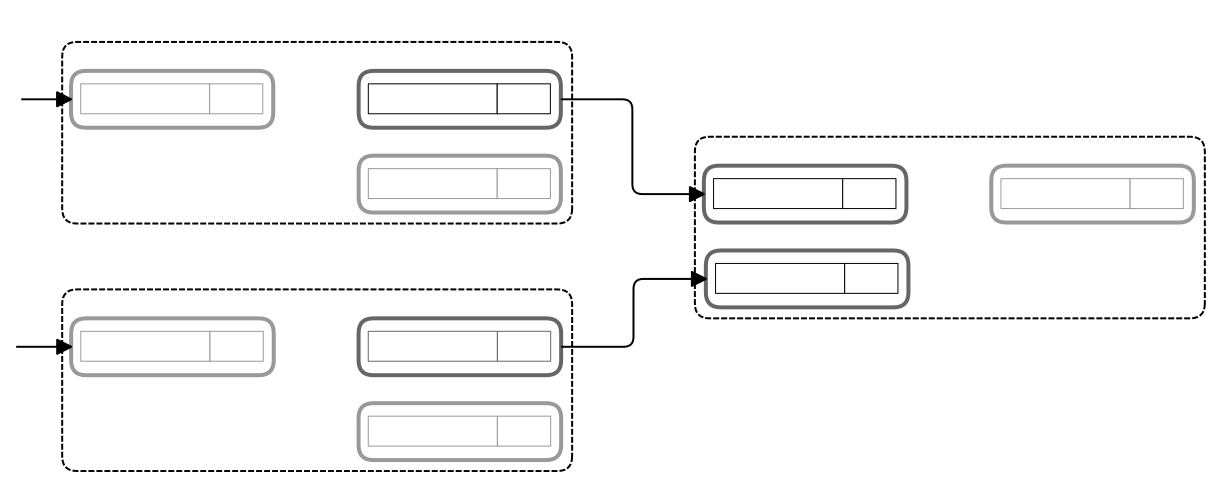
\includegraphics[width=\textwidth]{content/bitcoin/img/transactions2}
\caption{A chain of transactions, the available balance of address C is the sum of the output value located on transaction A and for address E is the sum of the output located on transaction B. Address C and E are owned by the same private key. The Final balance of Address G is 2 Bitcoins.}
\label{fig:transactions2}
\end{figure}

\end{document}